\documentclass{beamer}
\usepackage[normalem]{ulem}
\usepackage[style=authoryear, backend=biber]{biblatex}
\addbibresource{reference.bib}
\usepackage{amsmath}
\usepackage{graphicx}

\usetheme{Madrid}

\title{Rule-based Monetary Policy in China}
\author{Liming Lin}
\institute{Sciences Po Paris}
\date{October 2025}

\begin{document}

\begin{frame}
  \titlepage
\end{frame}



% NEW: Section for the introduction
\section{Introduction}

% Slide 1: Motivation and Research Question
\begin{frame}{Motivation and Research Question}
  \begin{itemize}
    \item \textbf{Motivation}
    \begin{itemize}
     \item China: The most significant economy but its monetary policy remains under-studied.
     \item Currently facing a severe post-COVID demand slowdown.
     \begin{itemize}  
        \item Housing market slump; Local government debt crisis.
        \item CPI stagnating around 0\%; PPI negative since late 2022.
     \end{itemize}
     \item The People's Bank of China (PBoC)'s policy response appears passive or constrained.
      \begin{itemize}  
        \item No explicit monetary policy rule to anchor expectations.
        \item Gradual and limited cuts to interest rates and reserve requirements ratio.
     \end{itemize}
    \end{itemize}
    \item \textbf{Research Question:}
    \begin{itemize}
        \item \textbf{How would the Chinese Economy have differed if the PBoC had followed an explicit, rule-based (e.g., NGDP and Inflation Targeting) monetary policy?}
    \end{itemize}
  \end{itemize}
  
\end{frame}


% Slide 2: Empirical Strategy (Combined)
\section{Empirical Strategy}
\begin{frame}{Empirical Strategy}
\begin{itemize}
    \item \textbf{Methodology:} Use the \textbf{semi-structural method} \parencite{McKayWolf2023,CaravelloEtAl2024} to simulate counterfactual monetary policy rules in China.
    \item This approach requires two ``sufficient statistics" instead of a full structural model, making it robust to the Lucas Critique.
   
    \item \textbf{Statistic 1: Reduced-Form Projections}
    \begin{itemize}
        \item \textbf{Purpose:} The economy's baseline forecast, capturing all ``fundamental" shocks (fiscal, demand, etc.) without needing to identify them individually.
        \item \textbf{Estimation:} We will estimate this using a \textbf{Reduced-Form VAR} on key Chinese macro variables.
        \item \textbf{Time Period}: Quarterly data from 2015 to 2025; for robustness, we will also use 2020-2025.
    \end{itemize}
  \end{itemize}
\end{frame}

\begin{frame}{Empirical Strategy}
\begin{itemize}
    \item \textbf{Statistic 2: Policy Causal Effects}
    \begin{itemize}
        \item \textbf{Estimation Method 1:}  High-Frequency Identification (HFI) approach, following \textcite{DasSong2023}.
        \begin{itemize}
        \item \textbf{Identification:} They defined a "shock" as the change in 1-year Interest Rate Swaps (IRS) on the exact day of a PBoC policy announcement. 
        \item \textbf{Policy Tracked:} Price-based (MLF, LPR) and quantity-based (RRR) tools, Quarterly Report from PBoC, exchange rate regime reforms, etc.
     \end{itemize}
     \item \textbf{Alternative HFI:} \textcite{HeEtAl2023} applied the two-stage HFI method developed by \textcite{BuRogersWu2021} to China using the rates of various types of Nonnegotiable Certificates of Deposit (NCDs).
     \item \textbf{Estimation Method 2:} \textcite{RomerRomer2004} shocks constructed from estimated monetary policy rules by \textcite{ChenXiaoZha2025}. 
     \begin{itemize}
     \item Price-based rule that changes interest rates identified through 7-day repo rate (R007).
     \end{itemize}
    \end{itemize}
    
    
\end{itemize}
\end{frame}


% Slide 3: The Counterfactual Simulation
\begin{frame}{Sample Results from the Great Recession \parencite{CaravelloEtAl2024}}
The simulation solves for the optimal sequence of policy interventions (Statistic 2) required to steer the economy's baseline forecast (Statistic 1) to the new counterfactual target (Inflation, NGDP, etc.)
\begin{figure}
    \centering
    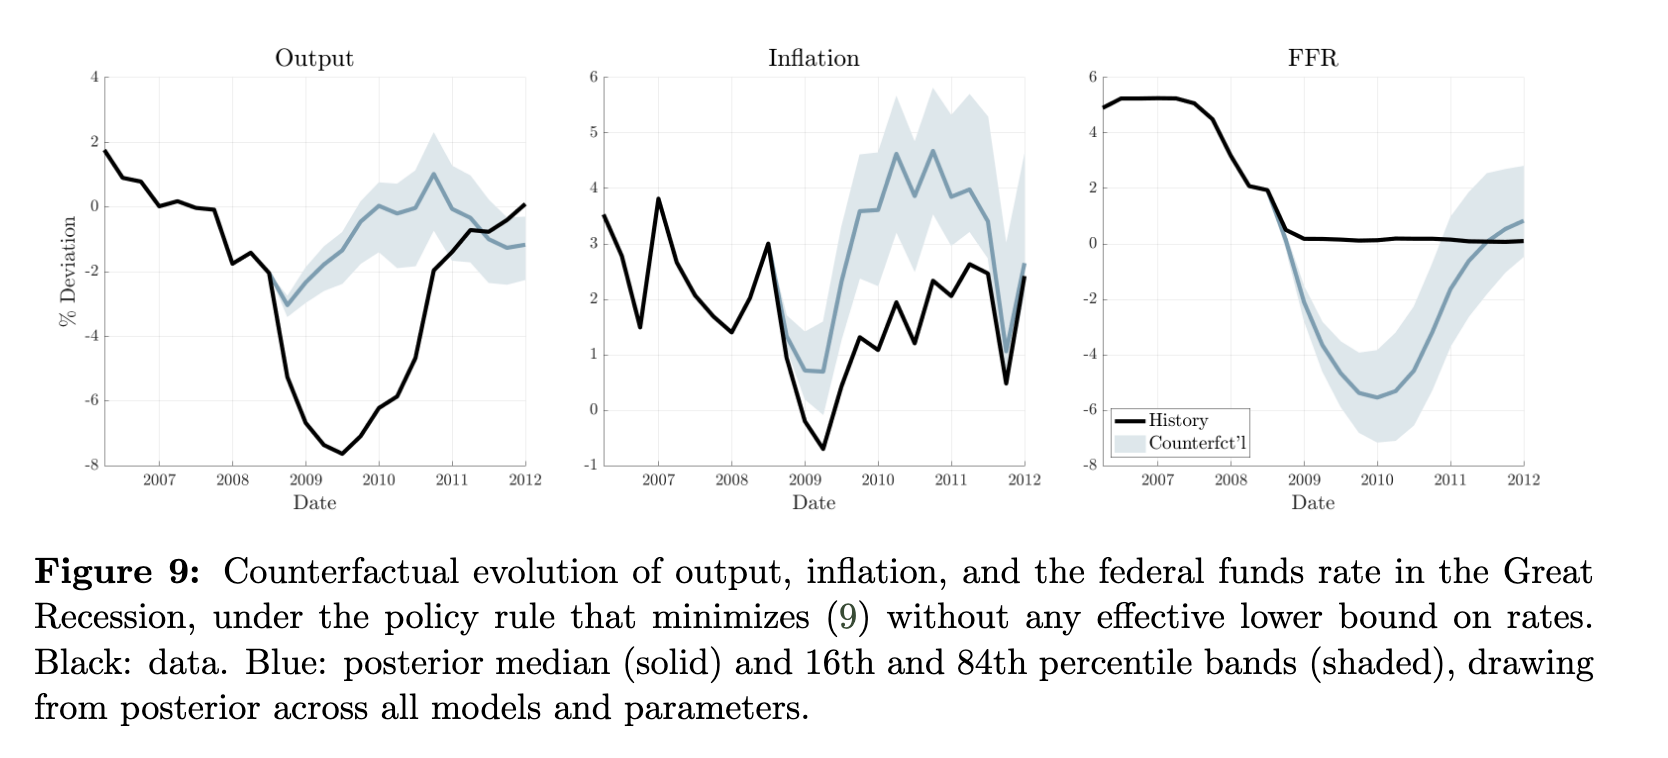
\includegraphics[width=1\textwidth]{Sample Results.png}
\end{figure}
\end{frame}

\begin{frame}{Limitations: Structural Applicability to China}
    While the focus on the MLF rate addresses the ``single instrument'' assumption, three structural challenges remain:

    \begin{itemize}
        \item \textbf{1. The Fiscal-Monetary Nexus (``Separation Principle'')}
        \begin{itemize}
            \item \emph{Model Assumption:} The private sector's structural equations are invariant to the policy rule.
            \item \emph{China Context:} Soft budget constraints (SOEs, LGFVs) create a quasi-fiscal channel. Aggressive counterfactual tightening could force structural breaks (e.g., fiscal bailouts), violating invariance.
        \end{itemize}
        
        \item \textbf{2. Information Asymmetry (``Signaling Channel'')}
        \begin{itemize}
            \item \emph{Model Assumption:} Policy actions do not reveal private information about the state of the economy.
            \item \emph{China Context:} Given lower data transparency, a PBOC rate hike might be interpreted as a signal of strong growth rather than tightening, reversing the intended effect.
        \end{itemize}

        \item \textbf{3. Availability of ``News Shocks''}
        \begin{itemize}
            \item \emph{Model Assumption:} Accurate counterfactuals require identifying ``news shocks'' (forward guidance) to span expectations.
            \item \emph{China Context:} Explicit forward guidance is historically limited. Weak identification of news shocks reduces the precision of ex-ante counterfactual enforcement.
        \end{itemize}
    \end{itemize}
\end{frame}


\section{Appendix}
\begin{frame}[plain]
  \vfill % Pushes content down from the top
  \centering % Centers content horizontally
  
  {\Huge \textbf{Appendix}} % Your text, made large and bold
  
  \vfill % Pushes content up from the bottom
\end{frame}

\begin{frame}
\frametitle{The Semi-Structural Method for Policy Counterfactuals}

\begin{itemize}
    \item \textbf{The Goal:} Evaluate policy counterfactuals (e.g., "what if the Fed had a different rule?") without committing to a fully specified structural model.


    \item \textbf{Core Insight:} A change in the policy \textit{rule} is equivalent to an appropriate, expected path of policy \textit{shocks} applied to the \textit{baseline} economy forecast.


   \item \textbf{Surviving the Lucas Critique:}
    \begin{itemize}
        \item The method models a systematic, \alert{fully expected} rule change, not a sequence of surprises.
        \item It uses a combination of date-0 shocks (contemporaneous + "news" shocks) to enforce the new rule in agents' expectations from the start.
    \end{itemize}

    
   \item \textbf{Key "Structural" Assumption (The Split):}
    \begin{itemize}
        \item The economy can be split into a \textbf{"non-policy block"} (private sector behavior) and a \textbf{"policy block"} (the rule).
        \item The non-policy block is assumed to be stable and depends \alert{only} on the \textit{path of the policy instrument} (e.g., the yield curve), not on the rule that generates it.
    \end{itemize}
\end{itemize}
\end{frame}

\section{Counterfactual Policy Rules}

\begin{frame}{Counterfactual Rules}
\textbf{1. Strict Inflation Targeting:}
\[
\min \mathcal{L} = \mathbb{E}_{0} \sum_{t=0}^{\infty} \beta^t \left[ (\pi_t - \pi_t^*)^2 \right]
\]

\textbf{2. Strict NGDP Targeting:}
\[
\min \mathcal{L} = \mathbb{E}_{0} \sum_{t=0}^{\infty} \beta^t \left[ (\Delta x_t - \Delta x_t^*)^2 \right]
\]

\textbf{3. Flexible Inflation Targeting:}
\[
\min \mathcal{L} = \mathbb{E}_{0} \sum_{t=0}^{\infty} \beta^t \left[ (\pi_t - \pi_t^*)^2 + \lambda_{y} (y_t - y_t^*)^2 \right]
\]

\textbf{4. Triple Mandate (PBoC-style):}
\begin{itemize}
    \item Includes the PBoC's explicit goal of currency stability.
    \[
    \min \mathcal{L} = \mathbb{E}_{0} \sum_{t=0}^{\infty} \beta^t \left[ (\pi_t - \pi_t^*)^2 + \lambda_{y} (y_t - y_t^*)^2 + \lambda_{e} (e_t - e_t^*)^2 \right]
    \]
\end{itemize}
\end{frame}


\begin{frame}{The Structural Part}
\begin{itemize}
    
    \item \textbf{Robustness Check / Future Work (The "Hybrid" Method):}
    \begin{itemize}
        \item \textbf{Problem:} If our baseline fails (or as a check), we can address the critique that the empirical "Recipe" is incomplete (i.e., missing "long-end" effects).
        \item \textbf{Check:} We can use a minimal structural model (e.g., a simple NK model) and "discipline" it by forcing its short-term IRF to match our HFI-estimated IRF but do not model shocks and monetary policy rules.
        \item We then use this "disciplined" model to extrapolate the long-term part of our "Recipe" and re-run the simulation.
    \end{itemize}
\end{itemize}
\end{frame}

\begin{frame}{How to Measure Chinese Output}
\begin{itemize}
    \item \textbf{The Challenge:} Official quarterly GDP data is famously smoothed, low-frequency and over-revised.
    \item \textbf{Primary Approach:} We may use the The China Cyclical Activity Tracker developed by the San Francisco Fed \parencite{FernaldHsuSpiegel2021}.
    \item \textbf{Robustness Checks:}
    \begin{itemize}
        \item Use other, well-measured monthly variables (like Industrial Production) as a simpler proxy.
    \end{itemize}
\end{itemize}
\end{frame}

\begin{frame}[allowframebreaks]{References}
    
    \printbibliography
\end{frame}
\end{document}
